%!TEX root = ./template-skripsi.tex
%-------------------------------------------------------------------------------
%                            BAB III
%               			PEMBAHASAN
%-------------------------------------------------------------------------------

\chapter{IMPLEMENTASI PROGRAM}


\section{Analisis Kebutuhan }
Pada tahapan ini, penulis mengumpulkan informasi tentang kebutuhan dari perangkat lunak yang akan dikembangkan dengan cara mewawancara beberapa pihak seperti Koordinator Program Studi, Tim Penjamin Mutu Prodi, dan Gugus Penjamin Mutu FMIPA yang dapat dilihat pada Lampiran A. Penulis juga mengumpulkan informasi dari pengumpulan data pada penelitian serupa yang sebelumnya pernah dilakukan yaitu penelitian yang dilakukan oleh \cite{FitriAndiniMedIrzal2017} yang berjudul "Perancangan dan Implementasi Sistem Absensi Online Berbasis Android di Linkungan Universitas Negeri Jakarta"  dan \cite{Kultsum2021} yang berjudul ''Rancang Bangun Sistem Presensi Akademik Berbasis Web Dengan \textit{Framework} Laravel di Lingkungan Program Studi Ilmu Komputer Universitas Negeri Jakarta''. Berikut beberapa hasil kebutuhan yang penulis dapatkan:

\begin{enumerate}
	\item Sistem memiliki lima jenis pengguna yaitu mahasiswa, penanggung jawab mata kuliah, dosen, tim penjamin mutu, dan admin.
	\item Mahasiswa dapat melihat kelas-kelas yang diambil, mengisi presensi ketika sudah ada pertemuan atau form 05 yang diisi oleh penanggung jawab atau dosen, dan melihat nilai tugas-tugas yang telah diisi oleh dosen.
	\item Penanggung jawab mata kuliah adalah bagian dari mahasiswa dengan tugas tambahan yaitu  mengisi atau memvalidasi form 05. Penanggung jawab mata kuliah dipilih oleh dosen pada pertemuan pertama.
	\item Dosen dapat melihat kelas-kelas yang diampu, mengisi form 05 untuk pertemuan pada kelas tersebut, dan dapat menutup waktu presensi untuk mahasiswa. Untuk memvalidasi presensi dari mahasiswa Dosen dapat memilih untuk memvalidasi semua presensi yang masuk, melakukan seleksi validasi presensi yang sudah masuk, atau memvalidasi semua presensi yang masuk sebelum waktu yang ditentukan.  Dosen juga dapat menambahkan tugas dan mengisi nilai tugas setiap mahasiswa dengan mengunduh format excel yang telah tersedia dan mengunggah \textit{file excel} tersebut ketika ada pembaruan. Ketika penanggung jawab mata kuliah tidak bisa hadir, dosen juga dapat menunjuk penanggung jawab mata kuliah sementara untuk pertemuan tersebut.
	\item Tim penjamin mutu adalah bagian dari dosen dengan tambahan yaitu memiliki menu monitoring yang berisi informasi semua kelas-kelas pada program studi termasuk yang tidak diampu oleh dosen tersebut. Tim penjamin mutu hanya dapat melihat form 05 dan form 06 tanpa bisa merubah data di dalamnya.
	\item Admin hanya memiliki satu tugas yaitu untuk mengatur atau mengubah jenis user dosen atau tim penjamin mutu jika ada perubahan.
	\item Satu kelas bisa diampu lebih dari satu dosen.
	
\end{enumerate}


\section{Implementasi Spiral}


Pada penelitian ini, penulis mengembangkan perangkat lunak dengan menggunakan proses model Spiral dimana pengembangan dilakukan dalam \emph{cycle} atau iterasi. Dari hasil analisis kebutuhan yang telah dilakukan, penulis mengambil beberapa diantaranya untuk dikembangkan dalam iterasi pertama. Total iterasi yang direncanakan adalah tiga iterasi dengan periode waktu satu hingga dua minggu per iterasi. Berikut adalah fase-fase yang penulis jalankan dalam iterasi pertama.

\section{Perencanaan}

Dalam tahap perencanaan, penulis membuat desain-desain dari beberapa kebutuhan yang telah didapatkan dalam bentuk \textit{Use Case Diagram}, \textit{Activity Diagram}, dan rancangan tampilan antarmuka untuk menjadi tujuan yang akan dikembangkan dalam iterasi yang dijalankan. Selain itu, dalam iterasi pertama penulis juga membuat desain rancangan sistem secara keseluruhan dalam bentuk \textit{Entity Relation Diagram}. Iterasi ini berjalan selama dua minggu.

%gambar use case
\subsection{Use Case Diagram}

Pada iterasi pertama, penulis mengembangkan sistem dari sisi mahasiswa terlebih dahulu dikarenakan penulis dapat mengakses \textit{web service} SIAKAD dengan akun mahasiswa penulis. Berikut adalah use case diagram yang telah dibuat:

\begin{figure}[H]
	\centering
	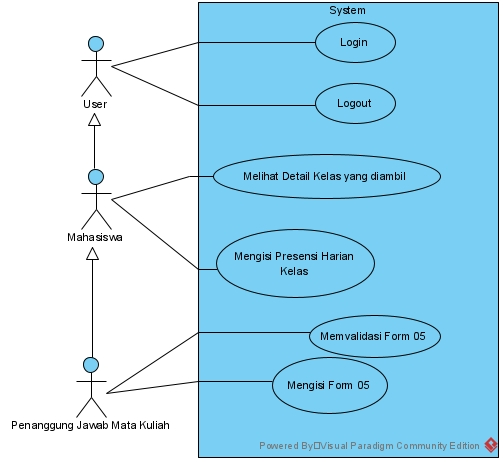
\includegraphics[width=0.8\textwidth]{gambar/diagram/Use Case Iteration 1}
	\caption{Desain \textit{Use Case Diagram Iterasi Pertama}}
	\label{fig:usecase1st}
\end{figure}

Aktor Mahasiswa dapat melihat detail kelas-kelas yang diambil seperti presensi dan nilai setiap mahasiswa pada kelas tersebut dan mengisi presensi pertemuan yang sedang berlangsung.
Aktor Penanggung Jawab Mata Kuliah dapat digeneralisasi menjadi aktor Mahasiswa sehingga mendapat wewenang yang sama seperti aktor Mahasiswa. Aktor penanggung jawab mata kuliah juga dapat mengisi form 05 atau memvalidasi form 05 yang telah dibuat oleh dosen dan memvalidasi presensi form 06 mahasiswa lain.

\subsection{Activity Diagram}

Dari beberapa \textit{use case} yang telah dibuat, penulis juga membuat \textit{activity diagram} untuk beberapa \textit{use case} yang butuh penjelasan alur untuk menjalankannya. Berikut adalah \textit{activity diagram} yang telah dibuat:

\begin{figure}[h!]
	\centering
	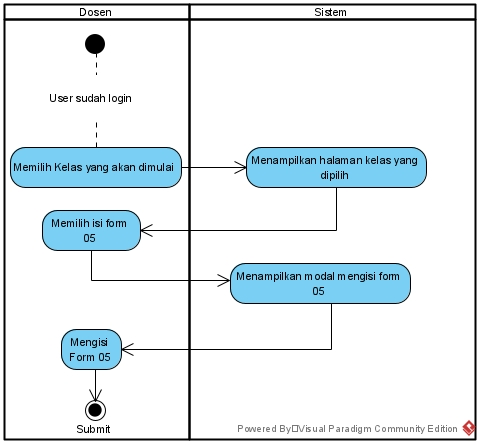
\includegraphics[width=0.7\textwidth]{gambar/diagram/Mengisi Form 05}
	\caption{\textit{Activity} Mengisi Form 05}
	\label{fig:activity2}
\end{figure}

\begin{figure}[h!]
	\centering
	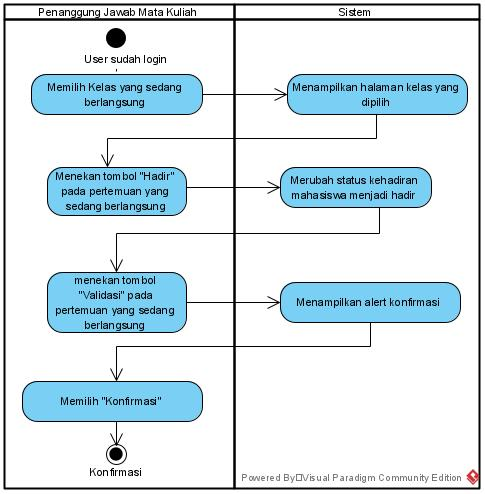
\includegraphics[width=0.7\textwidth]{gambar/diagram/Mengisi Presensi dan Memvalidasi Form 05}
	\caption{\textit{Activity} Mengisi Presensi dan Memvalidasi Form 05}
	\label{fig:activity1}
\end{figure}

Pada gambar \ref{fig:activity2} menggambarkan aktivitas mengisi form 05 yang dapat dilakukan oleh penanggung jawab mata kuliah dan dosen. Pada pengisiannya, penanggung jawab mata kuliah dapat mengosongkan terlebih dahulu materi pembelajaran untuk nantinya ditambahkan oleh dosen.
Pada gambar \ref{fig:activity1} menggambarkan aktivitas mengisi presensi yang dapat dilakukan oleh setiap mahasiswa dan memvalidasi form 05 yang dapat dilakukan oleh penanggung jawab dan dosen.

\subsection{Rancangan Tampilan Antarmuka}

Pada rancangan tampilan antar muka program, penulis membuat desain awal dengan menggunakan \textit{tools online}. Pada halaman \textit{login} yang dapat dilihat pada gambar \ref{fig:login}, user mengisi email dan \textit{password} yang terdaftar pada \textit{web service} SIAKAD.

\begin{figure}[h!]
	\centering
	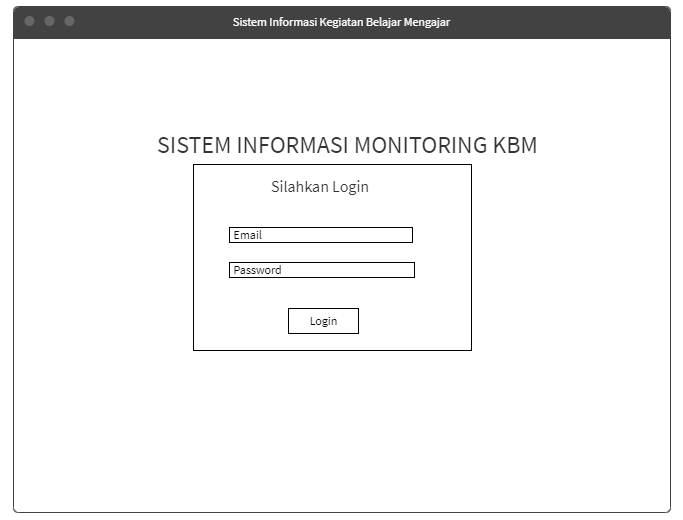
\includegraphics[width=0.8\textwidth]{gambar/mockup/login}
	\caption{Desain Halaman \textit{Login}}
	\label{fig:login}
\end{figure}

Setelah \textit{user} berhasil melakukan \textit{login}, \textit{user} akan dibawa ke halaman \textit{dashboard} dengan menu yang sedikit berbeda bagi setiap jenis \textit{user}. Pada \textit{user} mahasiswa yang dapat dilihat pada gambar \ref{fig:dashboard}, menu yang akan ditampilkan adalah \textit{Home}, Rekap Presensi, dan daftar kelas yang diambil oleh mahasiswa tersebut.

\begin{figure}[h!]
	\centering
	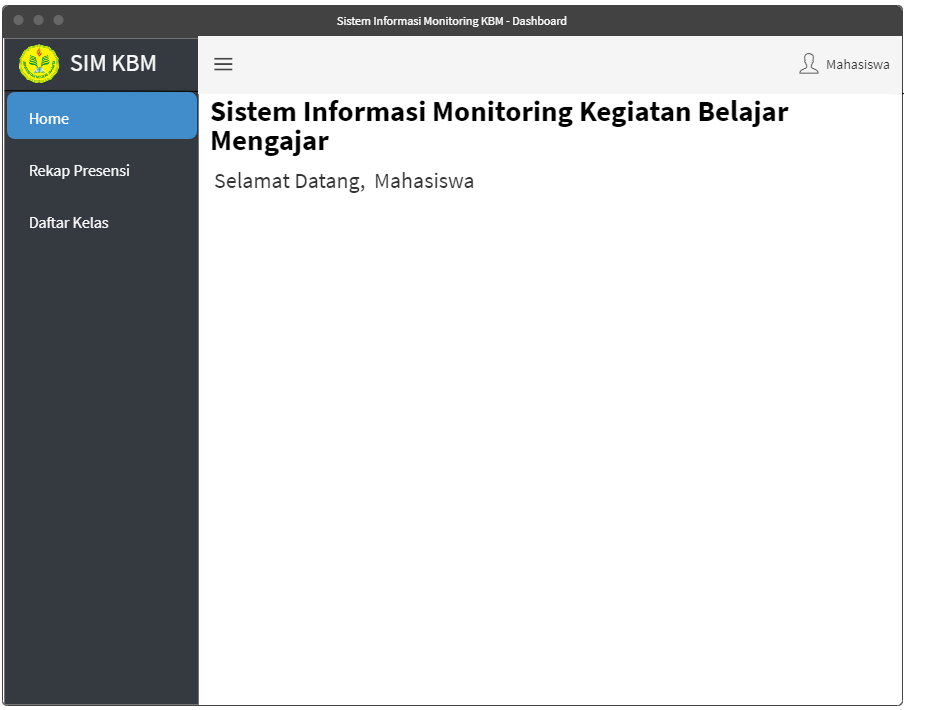
\includegraphics[width=0.8\textwidth]{gambar/mockup/home_mahasiswa}
	\caption{Desain Halaman \textit{Dashboard} Pada mahasiswa}
	\label{fig:dashboard}
\end{figure}


Menu Daftar Kelas merupakan menu yang digunakan untuk membuka halaman kelas yang diambil. Halaman Daftar Kelas dapat dilihat pada gambar \ref{fig:daftarkelas}. Menu kelas terdapat empat bagian \textit{tab} di dalamnya, yaitu Pertemuan, Presensi, Tugas, dan Nilai. Pada \textit{tab} pertemuan yang dapat dilihat pada gambar \ref{fig:form05dosen} dosen dapat menambah pertemuan, memvalidasi form yang dibuat oleh penanggung jawab, memvalidasi presensi mahasiswa, dan mengisi pokok bahasan yang dibahas pada pertemuan tersebut. Setelah pertemuan sudah dibuat dan mahasiswa sudah mengisi presensi, dosen juga bisa memvalidasi presensi mahasiswa tersebut. Pada \textit{tab} ini mahasiswa dapat memilih Hadir untuk mengisi presensi pada pertemuan tersebut yang bisa dilihat pada gambar \ref{fig:form05mhs}. Penanggung jawab mata kuliah memiliki fungsi yang sama dengan mahasiswa dan dosen.

\begin{figure}[h!]
	\centering
	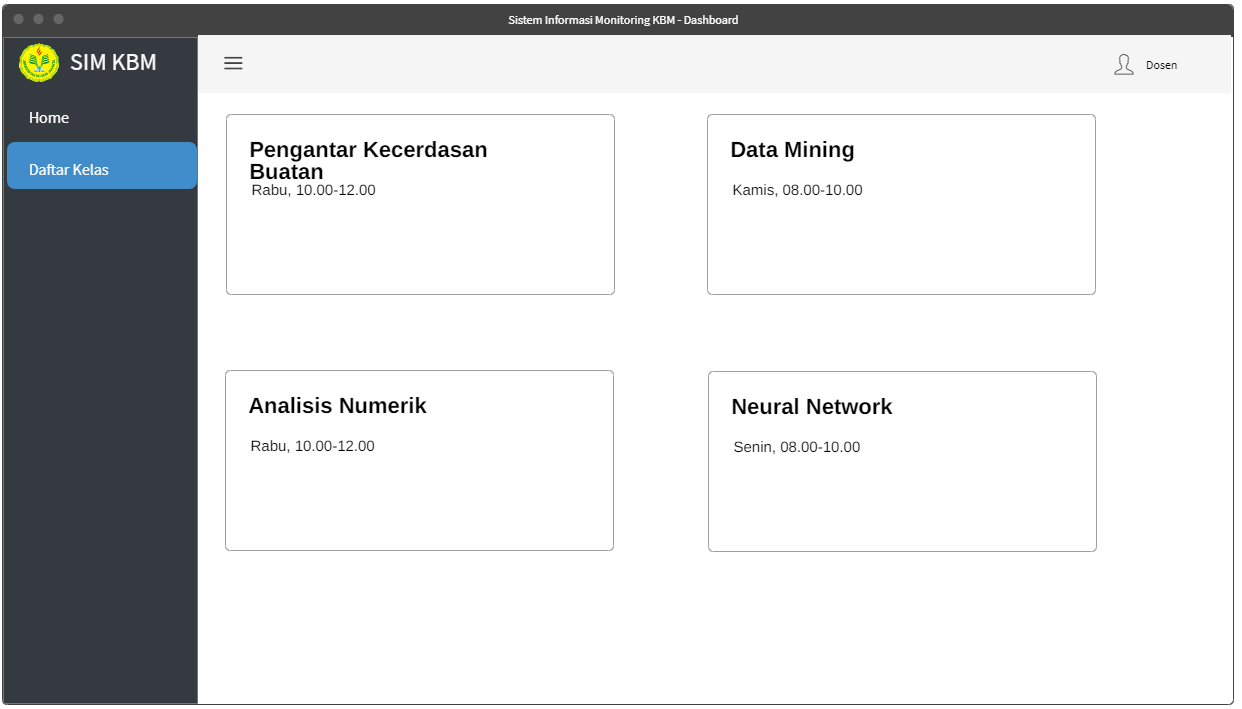
\includegraphics[width=0.8\textwidth]{gambar/mockup/daftar_kelas}
	\caption{Desain Halaman Daftar Kelas}
	\label{fig:daftarkelas}
\end{figure}

\begin{figure}[h!]
	\centering
	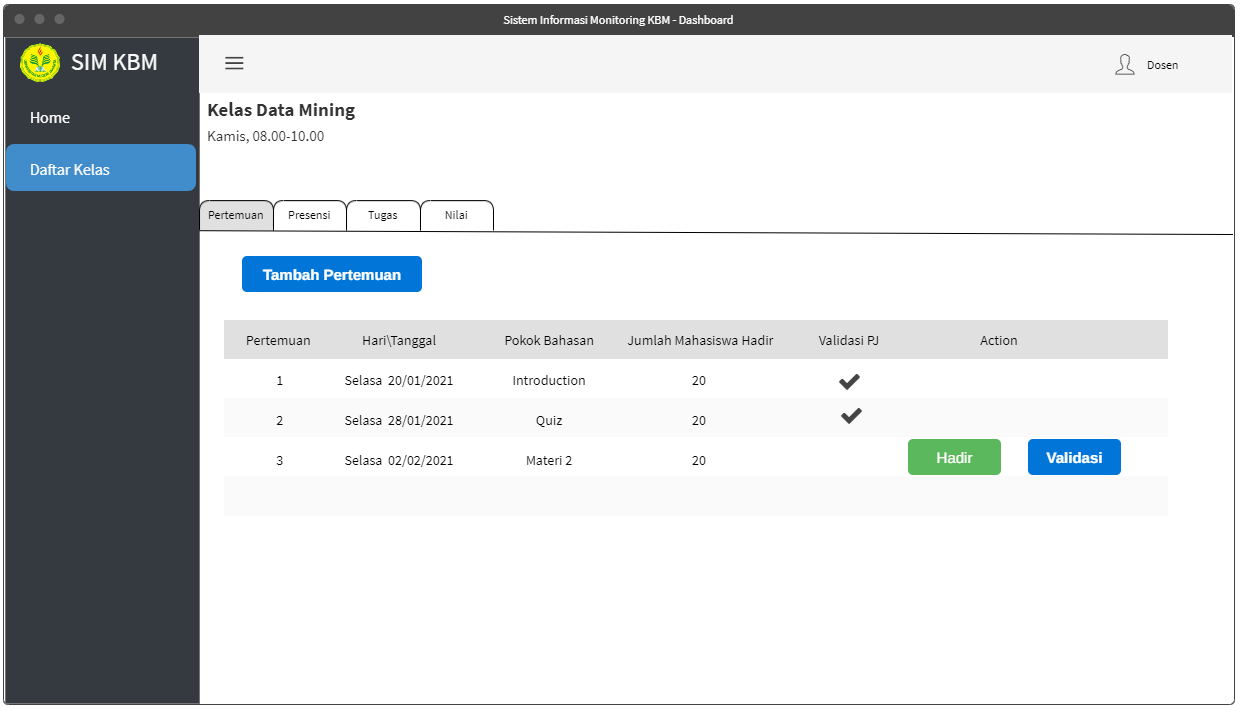
\includegraphics[width=0.8\textwidth]{gambar/mockup/form05_pj}
	\caption{Desain Halaman Form 05 Pada Penanggung Jawab}
	\label{fig:form05pj}
\end{figure}

\begin{figure}[h!]
	\centering
	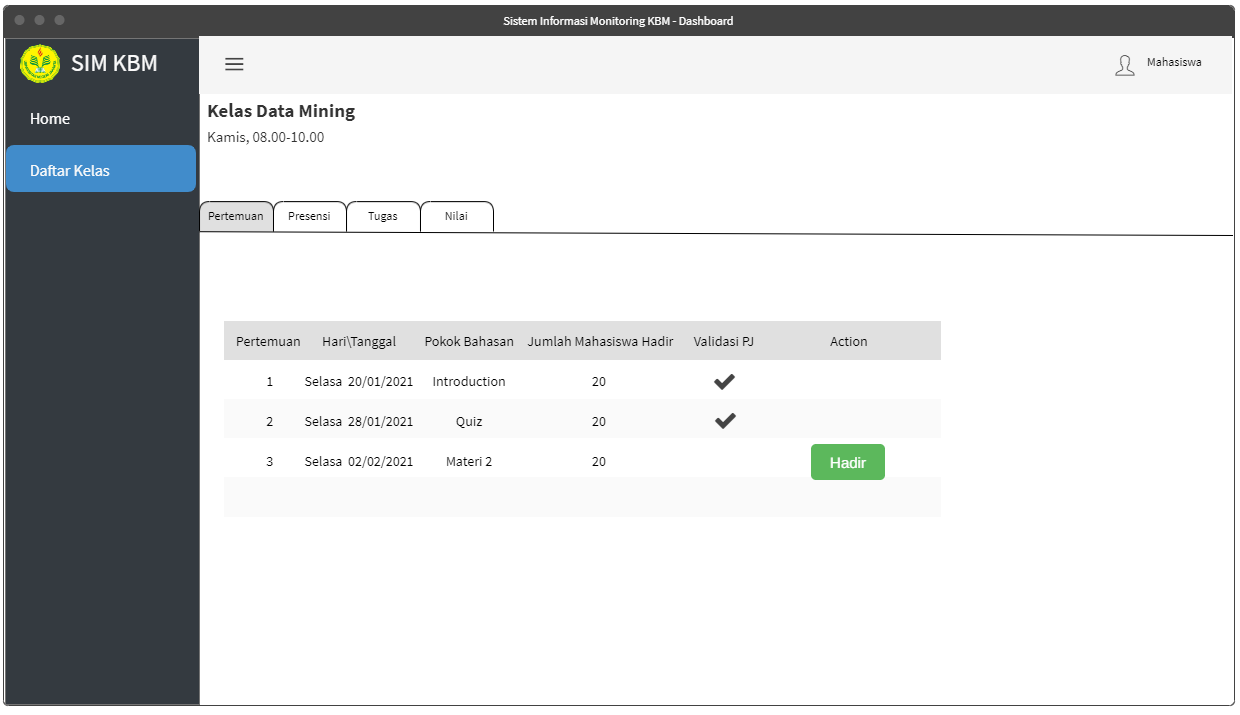
\includegraphics[width=0.8\textwidth]{gambar/mockup/form05_mahasiswa}
	\caption{Desain Halaman Form 05 Pada Mahasiswa }
	\label{fig:form05mhs}
\end{figure}


\subsection{\textit{Class Diagram}}
	Desain \textit{Class Diagram} pada sistem yang dibuat digambarkan dengan mengikuti konsep MVC dimana \textit{class} pada desain dibagi menjadi tiga jenis yaitu \textit{model}, \textit{view}, \textit{controller}. Pada penggunaannya \textit{class} \textit{model} dan \textit{controller} dibuat pada bagian \textit{backend} dengan menggunakan Laravel sedangkan \textit{class view} dibuat pada bagian \textit{frontend} dengan menggunakan \textit{Vue}. Pada diagram berikut ketiga jenis \textit{class} dibedakan dengan menggunakan warna yang berbeda yaitu biru untuk \textit{model}, hijau untuk \textit{view}, dan merah untuk \textit{controller}. Desain \textit{class diagram} pada sistem dapat dilihat pada gambar \ref{fig:classdiagram}

\begin{figure}[H]
	\centering
	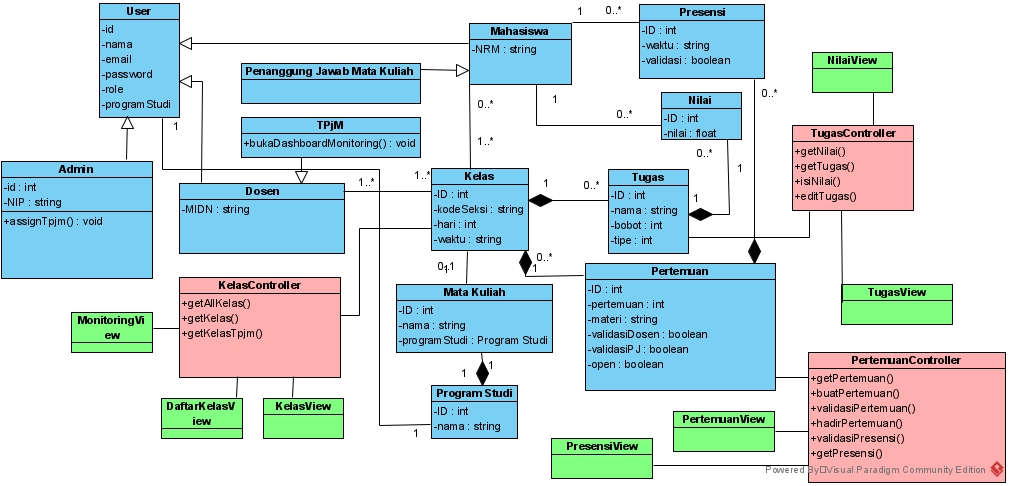
\includegraphics[width=1\textwidth]{gambar/diagram/Class Diagram Fix}
	\caption{Desain Class Diagram}
	\label{fig:classdiagram}
\end{figure}


\subsection{\textit{Entity Relationship Diagram}}
	Desain \textit{Entity Relationship Diagram} pada sistem ini dibuat menggambarkan setiap entitas yang digunakan dalam sistem dan relasinya pada \textit{database} dan pada \textit{web service} SIAKAD yang digunakan. Pada ERD tersebut terdapat sebelas entitas dimana enam diantaranya didapatkan dari \textit{web service} dan lima lainnya berada pada \textit{database} sistem ini sendiri. Entitas yang dibuat dan disimpan pada \textit{database} adalah entitas MahasiswaKelas. Absen, Pertemuan, Nilai, dan Tugas. Entitas MahasiswaKelas merupakan \textit{pivot} antara relasi mahasiswa dan kelas yang disimpan karena menyimpan informasi tambahan selain yang didapatkan dari \textit{webservice} yaitu nilai dan \textit{role} penanggung jawab. Entitas Pertemuan dan Absen yang menghubungkan antara mahasiswa dan kelas merupakan entitas yang menggambarkan form 05 dan 06. Desain ERD pada sistem dapat dilihat pada gambar \ref{fig:erd}

\begin{figure}[h!]
	\centering
	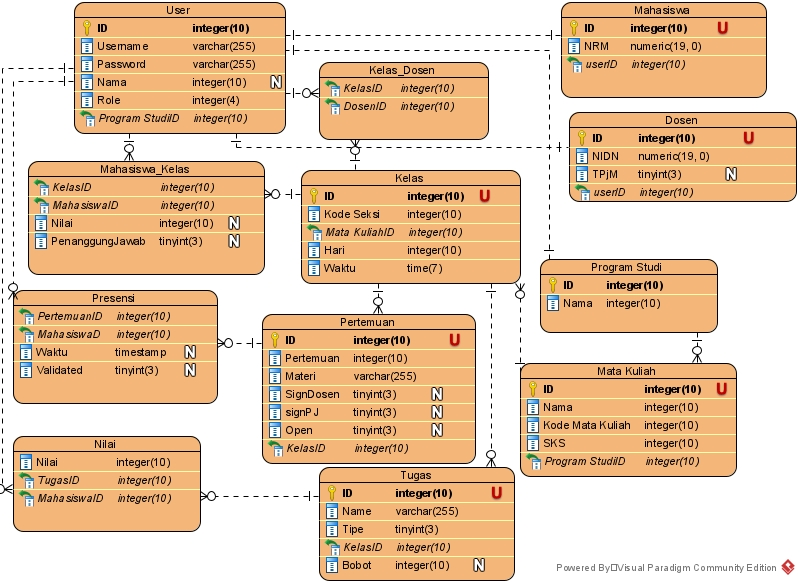
\includegraphics[width=1\textwidth]{gambar/diagram/Entity Relationship Diagram2}
	\caption{Desain Entity Relationship Diagram}
	\label{fig:erd}
\end{figure}

\section{Analisis Risiko}
	Pada fase selanjutnya, penulis melakukan analisis risiko yang dapat terjadi pada pengembangan perangkat lunak, dan mencoba mencari solusi yang dapat dilakukan untuk menangani risiko tersebut. Risiko-risiko yang telah teridentifikasi adalah sebagai berikut:
\begin{enumerate}
	\item Penulis tidak memiliki akses \textit{web service} SIAKAD sebagai dosen. 
	\item Relasi basis data yang tidak lengkap karena menggunakan data dari SIAKAD dan tidak menyimpan kembali ke basis data sistem.
	\item Tidak diberikannya dokumentasi dari \textit{web service} SIAKAD
\end{enumerate}
Setelah risiko yang mungkin terjadi teridentifikasi, penulis mendapat beberapa solusi yaitu:
\begin{enumerate}
	\item Meminta dibuatkan akun dosen dan kelas \textit{dummy} untuk melakukan pengembangan pada sisi dosen.
	\item Menggunakan \textit{query} manual untuk mengakses relasi pada basis data.
	\item Membuat list kebutuhan \textit{web service} dan berkomunikasi dengan pihak UPT TIK terkait \textit{web service} yang dibutuhkan.
\end{enumerate}

\section{Pengembangan}
	Pada fase pengembangan, penulis melakukan proses pengkodean sekaligus pengujian fitur yang dikembangkan. Hasil dari fase ini adalah perangkat lunak sesuai dengan tujuan yang telah ditentukan. Sebagai fase pertama penulis mulai dengan membuat basis data yang dibutuhkan, lalu membuat \textit{backend} beserta hubungannya dengan \textit{web service} SIAKAD, dan membuat \textit{frontend} atau tampilan.

\section{Evaluasi}
	Pada fase evaluasi, penulis melakukan \textit{review} atas iterasi yang telah dilakukan dan merencanakan iterasi yang selanjutnya. Untuk iterasi selanjutnya penulis akan mempersingkat waktu iterasi dengan menyelesaikan iterasi tanpa menunggu berakhirnya minggu kedua ketika semua tujuan iterasi sudah tercapai. Pada iterasi selanjutnya penulis akan mengembangkan sisi dosen dan menyempurnakan sisi mahasiswa yang telah dibuat.














\begin{comment}
\section{Desain Sistem}
Dalam tahapan ini, penulis membuat desain atau \textit{blueprint} dengan menggunakan UML(\textit{Unified Modelling Language}) dari hasil analisis kebutuhan pada tahap sebelumnya. Diagram-diagram yang dibuat oleh penulis adalah \textit{Use Case Diagram}, \textit{Activity Diagram}, dan \textit{Class Diagram}. Selain dari diagram-diagram UML tersebut, penulis juga membuat desain \textit{Entity Relationship Diagram} dan \textit{mockup} dari tampilan antar muka program. Penulis membuat semua diagram-diagram berikut dengan menggunakan Visual Paradigm.

\subsection{\textit{Use Case Diagram}}
	\textit{Use Case Diagram} menggambarkan interaksi apa saja yang dapat dilakukan oleh setiap jenis \textit{user} yang ada pada sistem yang dikembangkan oleh penulis. Pada sistem yang dibuat terdapat 5 aktor yaitu Mahasiswa, Penanggung Jawab Mata Kuliah , Dosen, TPjM, dan admin. Kelima aktor tersebut dapat digeneralisasi menjadi aktor \textit{User} dimana aktor \textit{User} harus melakukan \textit{login} sebelum mengakses sistem. Desain Use Case Diagram untuk sistem yang akan dibuat ada pada pada Gambar \ref{fig:form05}.
	
	Aktor Mahasiswa dapat melihat detail kelas-kelas yang diambil seperti presensi dan nilai setiap mahasiswa pada kelas tersebut dan mengisi presensi pertemuan yang sedang berlangsung.

	Aktor Penanggung Jawab Mata Kuliah dapat digeneralisasi menjadi aktor Mahasiswa sehingga mendapat wewenang yang sama seperti aktor Mahasiswa. Aktor penanggung jawab mata kuliah juga dapat mengisi form 05 atau memvalidasi form 05 yang telah dibuat oleh dosen dan memvalidasi presensi form 06 mahasiswa lain.

	Aktor Dosen memiliki wewenang yang hampir sama dengan wewenang khusus penanggung jawab mata kuliah seperti mengisi form 05, memvalidasi form 05, dan memvalidasi presensi harian kelas. Aktor dosen juga memiliki wewenang tambahan seperti membuat tugas, mengisi nilai, dan memilih penanggung jawab pengganti jika penanggung jawab tidak dapat melakukan tugasnya.

	Aktor TPjM dapat digeneralisasi menjadi aktor dosen sehingga memiliki wewenang  aktor dosen dengan tambahan  dapat melihat rangkuman performa semua kelas dan melihat detail kelas-kelas lain di program studi yang tidak diampu olehnya.

	

\begin{figure}[H]
	\centering
	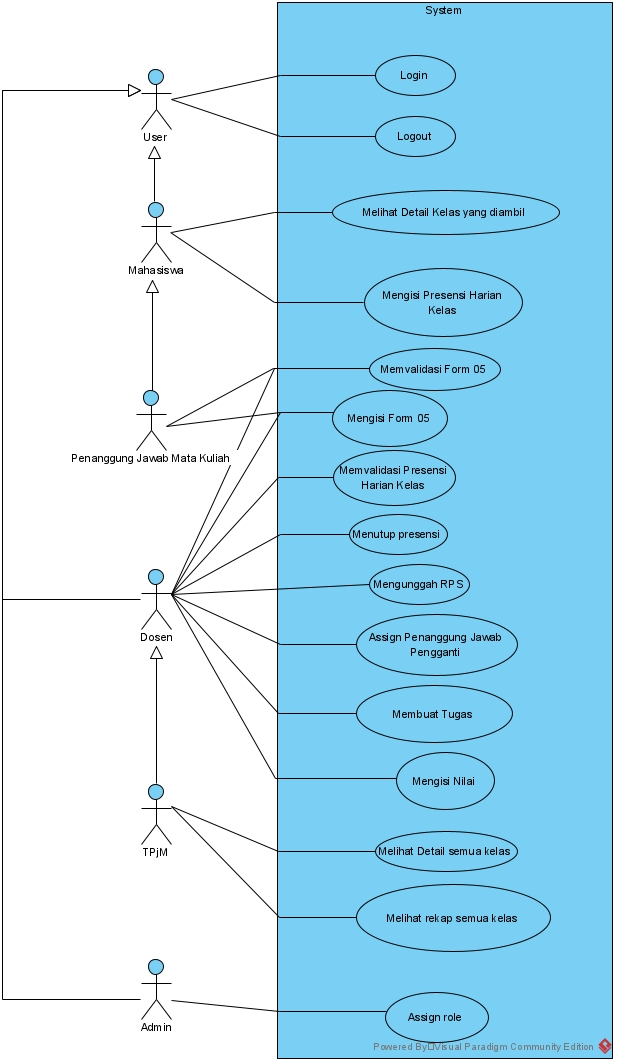
\includegraphics[width=0.8\textwidth]{gambar/diagram/Use Case Diagram}
	\caption{Desain \textit{Use Case Diagram}}
	\label{fig:form05}
\end{figure}

Aktor admin adalah aktor yang dapat mengganti \textit{role user-user} lainnya jika terjadi perubahan. Aktor admin juga bertanggung jawab untuk melakukan \textit{import} data pada awal semester.

\subsection{\textit{Activity Diagram}}
	\textit{Acitivity Diagram} menggambarkan bagaimana alur menjalankan aktivitas yang ada pada sistem. Pada desain sistem ini, dibuat beberapa diagram yang menggambarkan aktivitas-aktivitas utama yang dapat dilakukan pada sistem ini, yaitu mengisi presensi, memvalidasi form, membuat tugas, mengunggah nilai, mengunggah rps, dan memvalidasi presensi.

	Pada gambar \ref{fig:activity1} menggambarkan aktivitas mengunggah RPS dan menambah form 05 yang dapat dilakukan oleh dosen. Dosen diharuskan untuk mengunggah RPS pada pertemuan awal perkuliahan untuk dapat diakses oleh mahasiswa yang mengambil mata kuliah tersebut dan Tim Penjamin Mutu sebagai bahan evaluasi kesesuaian jalannya mata kuliah dengan RPS. Jika pada mata kuliah tersebut sudah memiliki RPS, dosen bisa langsung menambahkan form 05 dan memulai kelas. Form 05 dibutuhkan untuk membuka kesempatan mahasiswa mengisi presensi pertemuan tersebut.

\begin{figure}[h!]
	\centering
	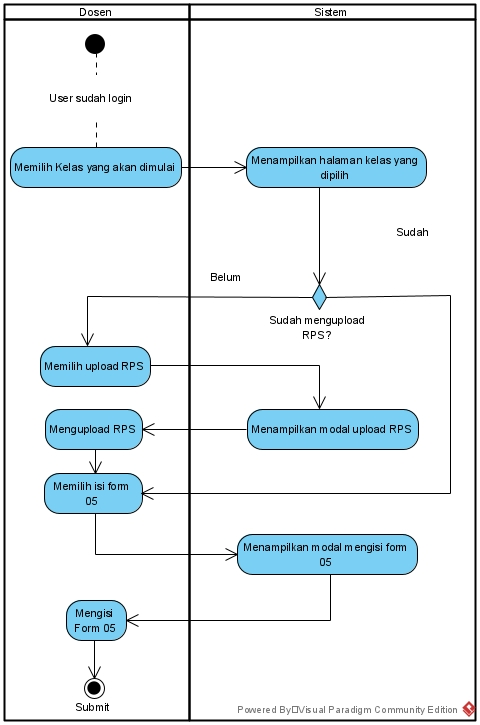
\includegraphics[width=0.7\textwidth]{gambar/diagram/Mengunggah RPS dan Menambah Form 05}
	\caption{\textit{Activity} Mengunggah RPS dan Menambah Form 05}
	\label{fig:activity1}
\end{figure}

	Pada gambar \ref{fig:activity2} menggambarkan aktivitas membuat tugas dan mengunggah nilai yang dapat dilakukan oleh dosen. Dosen dapat membuat tugas dengan cara menekan tombol tambah tugas dan mengisi nama tugas, tanggal, dan tipe tugas. Tipe tugas merupakan pilihan antara tugas, UTS, dan UAS. Tanggal tugas merupakan tanggal tugas tersebut diberikan dan dapat diubah jika tugas tersebut sudah diberikan kepada mahasiswa sebelumnya dan baru dimasukkan ke sistem. Dosen dapat mengunggah nilai dengan cara mengunduh \textit{template} nilai yang merupakan \textit{file} yang sudah berisi tabel nama-nama mahasiswa dan kolom-kolom kosong untuk nilai-nilai tugas, UTS, dan UAS. Dosen dapat mengisi file excel tersebut lalu diunggah kembali ke sistem untuk memperbarui nilai pada sistem.

\begin{figure}[h!]
	\centering
	\includegraphics[width=0.7\textwidth]{gambar/diagram/Membuat Tugas dan Mengunggah Nilai}
	\caption{\textit{Activity} Membuat Tugas dan Mengunggah Nilai}
	\label{fig:activity2}
\end{figure}

	Pada gambar \ref{fig:activity3} menggambarkan aktivitas mengisi presensi yang dapat dilakukan oleh mahasiswa dan memvalidasi form 05 yang dapat dilakukan oleh penanggung jawab mata kuliah. Mahasiswa dapat mengisi presensi dengan cara membuka halaman kelas yang sedang berlangsung dan menekan tombol Hadir. Presensi mahasiswa tersebut akan menunggu validasi oleh dosen untuk dianggap valid dan terekam oleh sistem. Penanggung Jawab Mata Kuliah diharuskan melakukan validasi form 05 yang telah dibuat oleh dosen dengan cara menekan tombol validasi pada tabel form 05 tersebut.

\begin{figure}[h!]
	\centering
	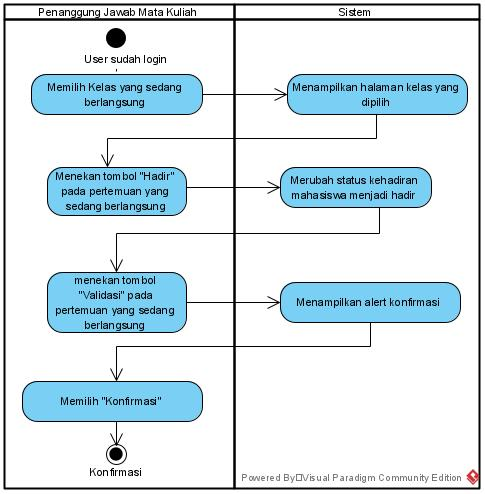
\includegraphics[width=0.7\textwidth]{gambar/diagram/Mengisi Presensi dan Memvalidasi Form 05}
	\caption{\textit{Activity} Mengisi Presensi dan Memvalidasi Form 05}
	\label{fig:activity3}
\end{figure}

	Pada gambar \ref{fig:activity4} menggambarkan aktivitas memilih penanggung jawab pengganti yang dapat dilakukan oleh dosen jika penanggung jawab mata kuliah tidak hadir pada pertemuan yang sedang berlangsung untuk memvalidasi form 05 yang telah dibuat. Penanggung jawab pengganti bersifat sementara dan hanya berlaku pada pertemuan tersebut.

\begin{figure}[h!]
	\centering
	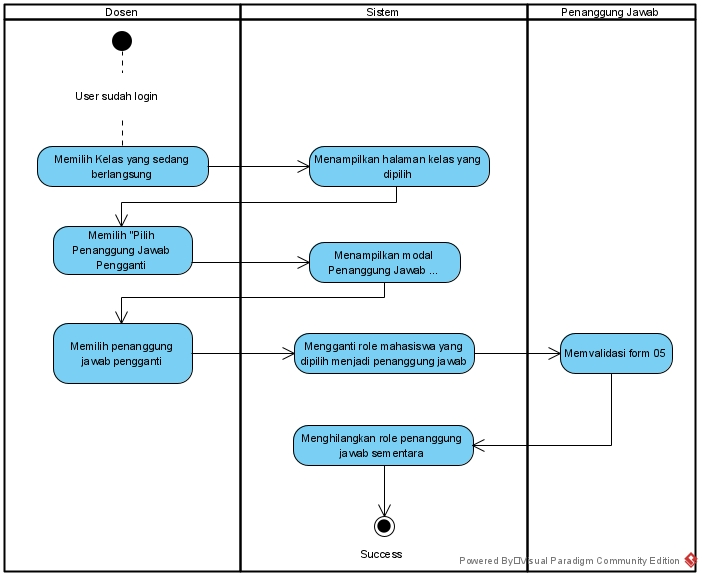
\includegraphics[width=0.7\textwidth]{gambar/diagram/Assign Penanggung Jawab Pengganti}
	\caption{\textit{Activity} Memilih Penanggung Jawab Pengganti}
	\label{fig:activity4}
\end{figure}
	
	Pada gambar \ref{fig:activity6} menggambarkan aktivitas mengganti \textit{role user} yang dapat dilakukan oleh admin. Aktivitas ini utamanya digunakan untuk mengganti \textit{role} TPjM yang dapat berganti setiap tahunnya.

	Pada gambar \ref{fig:activity5} menggambarkan aktivitas memvalidasi presensi yang dapat dilakukan oleh dosen. Dosen harus memvalidasi presensi mahasiswa agar presensi tersebut valid dan terekam oleh sistem. Dosen dapat memilih untuk memvalidasi semua presensi yang sudah diisi oleh mahasiswa atau memilih presensi yang tidak valid dengan cara membatalkan tanda centang \textit{checkbox} pada \textit{list} presensi yang akan divalidasi.

\begin{figure}[H]
	\centering
	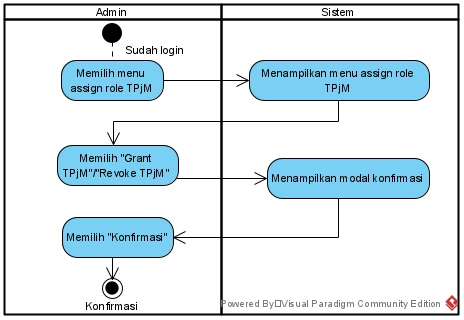
\includegraphics[width=0.7\textwidth]{gambar/diagram/Admin Assign Role}
	\caption{\textit{Activity} Mengganti \textit{role user}}
	\label{fig:activity6}
\end{figure}

\begin{figure}[H]
	\centering
	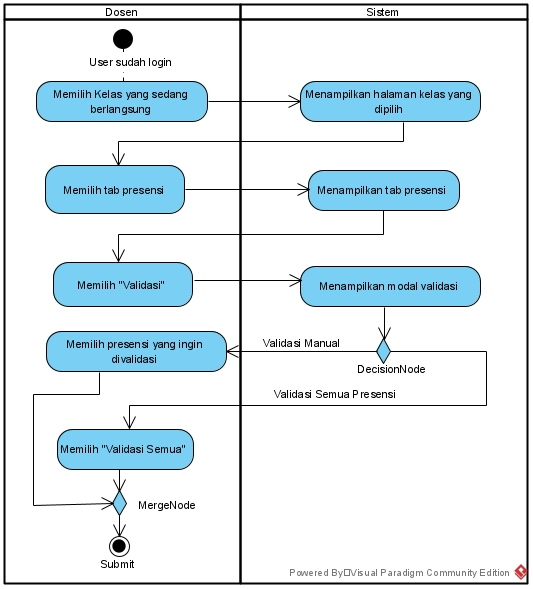
\includegraphics[width=0.7\textwidth]{gambar/diagram/Memvalidasi presensi}
	\caption{\textit{Activity} Memvalidasi Presensi}
	\label{fig:activity5}
\end{figure}



\subsection{\textit{Class Diagram}}
	Desain \textit{Class Diagram} pada sistem yang dibuat digambarkan dengan mengikuti konsep MVC dimana \textit{class} pada desain dibagi menjadi tiga jenis yaitu \textit{model}, \textit{view}, \textit{controller}. Pada penggunaannya \textit{class} \textit{model} dan \textit{controller} dibuat pada bagian \textit{backend} dengan menggunakan Laravel sedangkan \textit{class view} dibuat pada bagian \textit{frontend} dengan menggunakan \textit{Vue}. Pada diagram berikut ketiga jenis \textit{class} dibedakan dengan menggunakan warna yang berbeda yaitu biru untuk \textit{model}, hijau untuk \textit{view}, dan merah untuk \textit{controller}. Desain \textit{class diagram} pada sistem dapat dilihat pada gambar \ref{fig:classdiagram}

\begin{figure}[H]
	\centering
	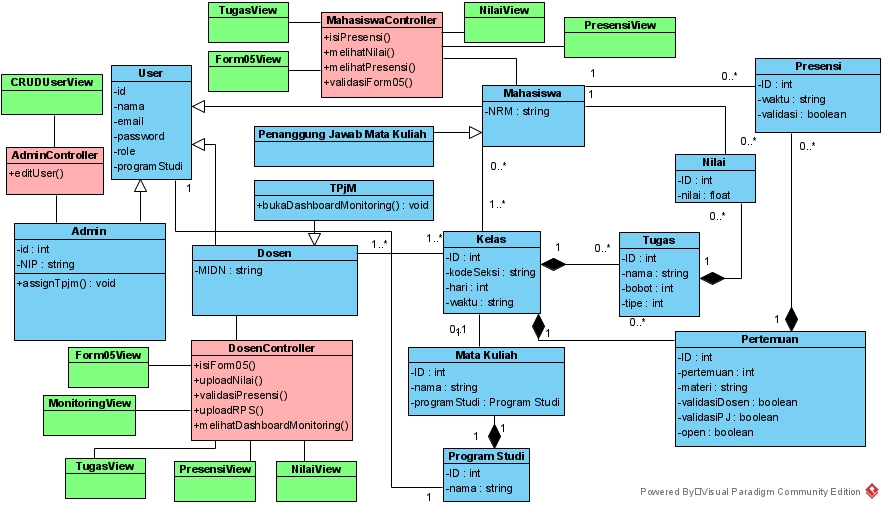
\includegraphics[width=1\textwidth]{gambar/diagram/Class Diagram}
	\caption{Desain Class Diagram}
	\label{fig:classdiagram}
\end{figure}

\subsection{\textit{Entity Relationship Diagram}}
	Desain \textit{Entity Relationship Diagram} pada sistem ini dibuat menggambarkan setiap entitas yang digunakan dalam sistem dan relasinya pada \textit{database} dan pada \textit{web service} SIAKAD yang digunakan. Pada ERD tersebut terdapat sebelas entitas dimana enam diantaranya didapatkan dari \textit{web service} dan lima lainnya berada pada \textit{database} sistem ini sendiri. Entitas yang dibuat dan disimpan pada \textit{database} adalah entitas MahasiswaKelas. Absen, Pertemuan, Nilai, dan Tugas. Entitas MahasiswaKelas merupakan \textit{pivot} antara relasi mahasiswa dan kelas yang disimpan karena menyimpan informasi tambahan selain yang didapatkan dari \textit{webservice} yaitu nilai dan \textit{role} penanggung jawab. Entitas Pertemuan dan Absen yang menghubungkan antara mahasiswa dan kelas merupakan entitas yang menggambarkan form 05 dan 06. Desain ERD pada sistem dapat dilihat pada gambar \ref{fig:erd}

\begin{figure}[h!]
	\centering
	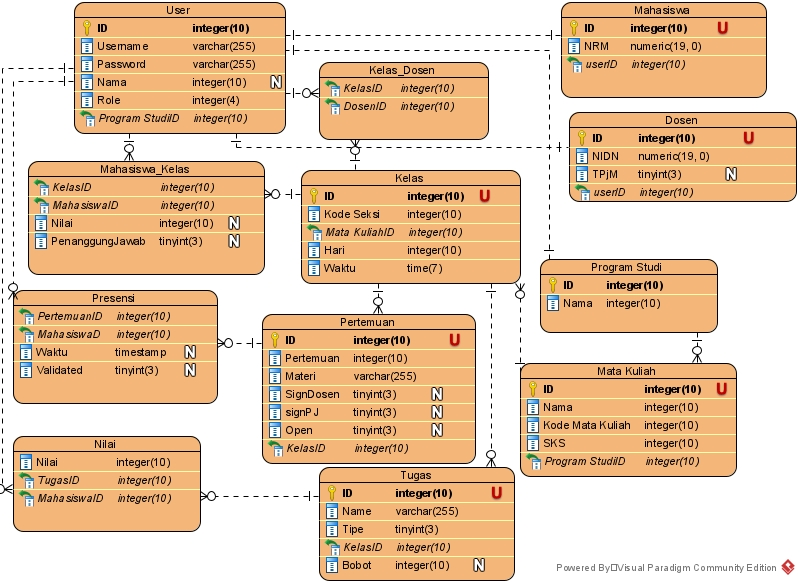
\includegraphics[width=1\textwidth]{gambar/diagram/Entity Relationship Diagram2}
	\caption{Desain Entity Relationship Diagram}
	\label{fig:erd}
\end{figure}

\subsection{Rancangan Tampilan Antarmuka Program}
	Pada rancangan tampilan antar muka program, penulis membuat desain awal dengan menggunakan \textit{tools online}. Pada halaman \textit{login} yang dapat dilihat pada gambar \ref{fig:login}, user mengisi email dan \textit{password} yang terdaftar pada \textit{web service} SIAKAD.

\begin{figure}[h!]
	\centering
	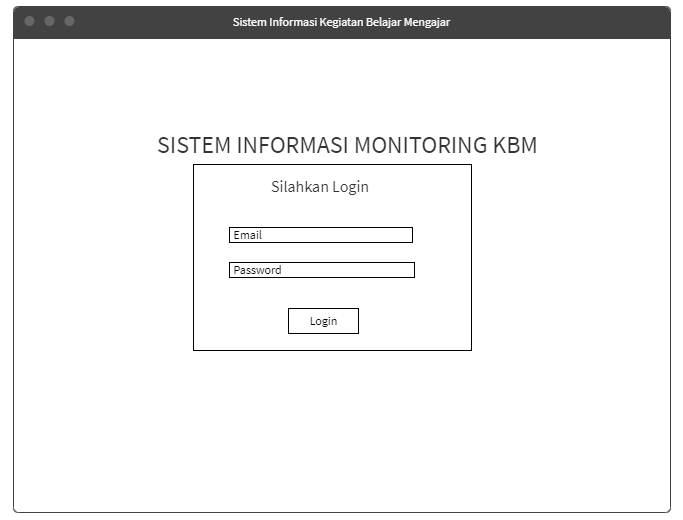
\includegraphics[width=0.8\textwidth]{gambar/mockup/login}
	\caption{Desain Halaman \textit{Login}}
	\label{fig:login}
\end{figure}

Setelah \textit{user} berhasil melakukan \textit{login}, \textit{user} akan dibawa ke halaman \textit{dashboard} dengan menu yang sedikit berbeda bagi setiap jenis \textit{user}. Pada \textit{user} mahasiswa yang dapat dilihat pada gambar \ref{fig:dashboard}, menu yang akan ditampilkan adalah \textit{Home}, Rekap Presensi, dan daftar kelas yang diambil oleh mahasiswa tersebut. Pada \textit{user} dosen, menu yang akan ditampilkan adalah \textit{Home} dan daftar kelas yang diampu oleh dosen tersebut. Pada \textit{user} TPjM menu tambahan akan ditampilkan berupa \textit{Monitoring}.

\begin{figure}[h!]
	\centering
	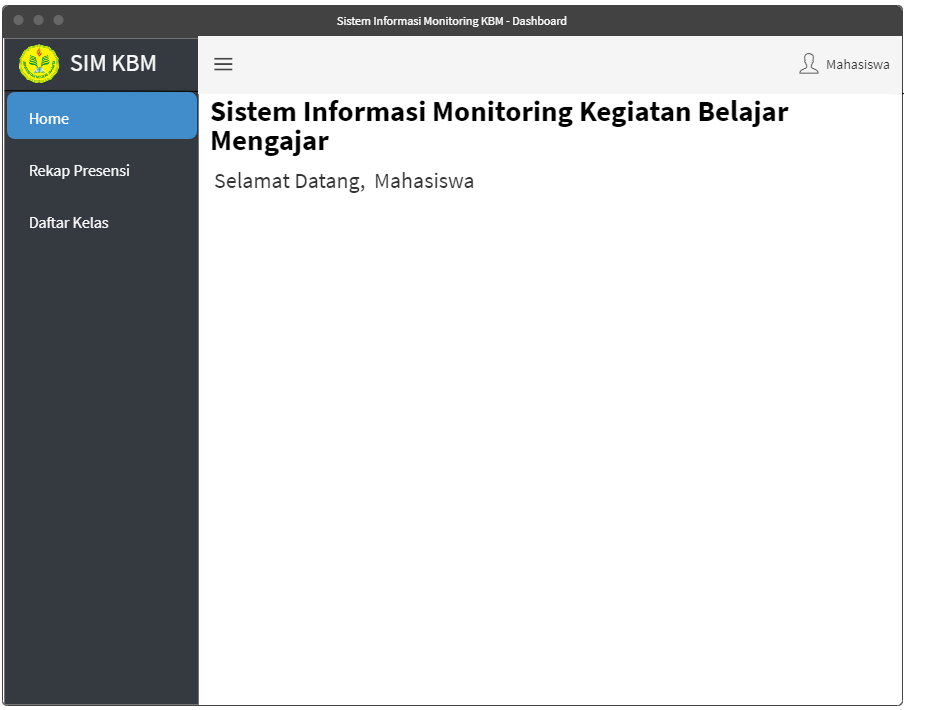
\includegraphics[width=0.8\textwidth]{gambar/mockup/home_mahasiswa}
	\caption{Desain Halaman \textit{Dashboard} Pada mahasiswa}
	\label{fig:dashboard}
\end{figure}

Pada menu Rekap Presensi yang dapat dilihat pada gambar \ref{fig:rekap}, mahasiswa dapat melihat rekap dari presensi setiap mata kuliah yang diambil yang tergabung menjadi satu. Pada menu \textit{monitoring} yang dapat dilihat pada gambar \ref{fig:monitoring}, TPjM dapat melihat daftar semua kelas yang ada pada program studi dan jumlah pertemuan yang telah berjalan. TPjM juga dapat membuka halaman kelas tersebut untuk melihat informasi di dalamnya hanya untuk melakukan monitoring tanpa bisa berinteraksi kecuali jika kelas tersebut juga diampu oleh TPjM tersebut.

\begin{figure}[h!]
	\centering
	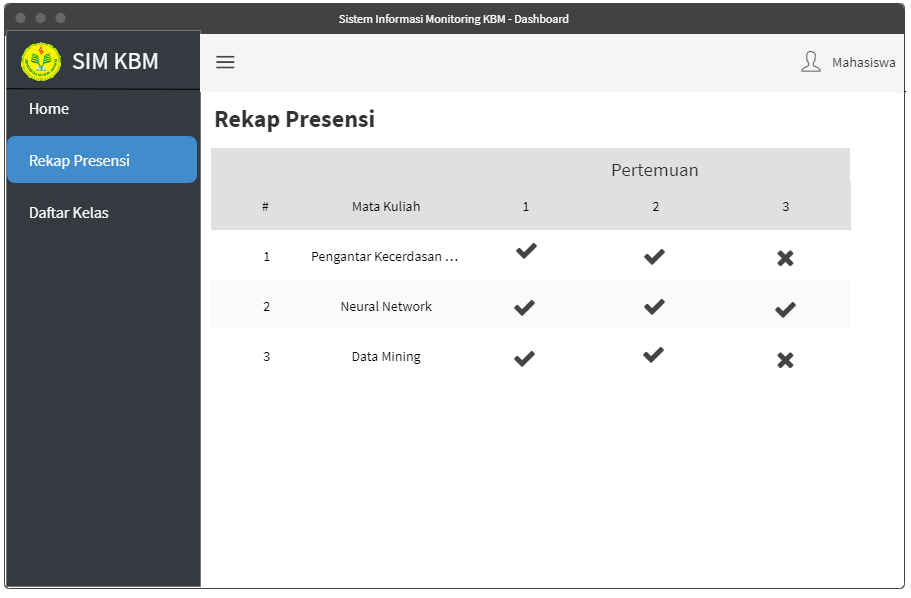
\includegraphics[width=0.8\textwidth]{gambar/mockup/rekap_presensi}
	\caption{Desain Halaman Rekap Presensi}
	\label{fig:rekap}
\end{figure}

\begin{figure}[h!]
	\centering
	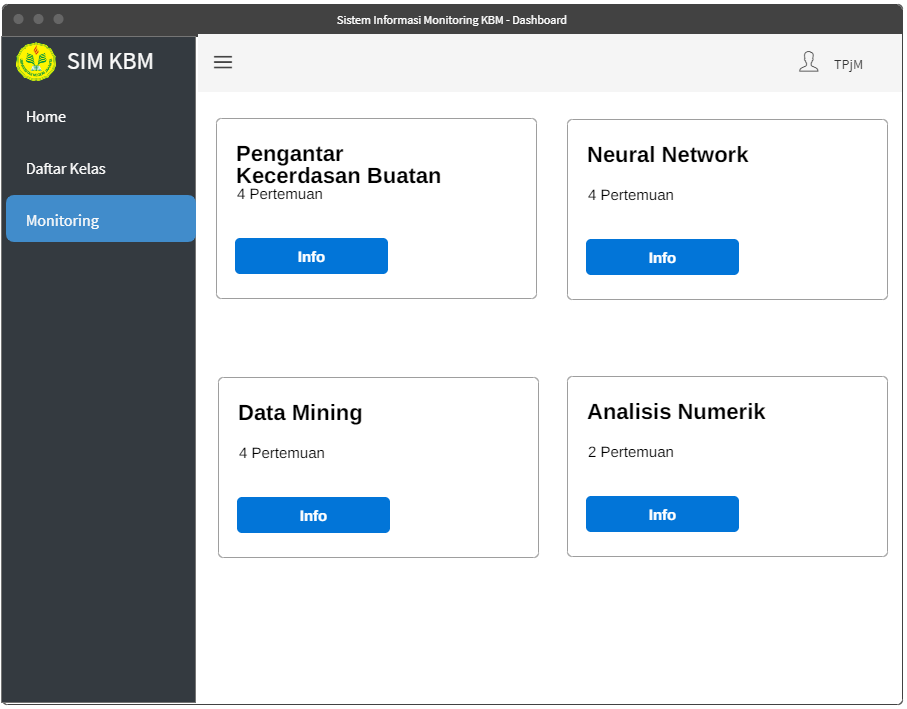
\includegraphics[width=0.8\textwidth]{gambar/mockup/monitoring}
	\caption{Desain Halaman \textit{Monitoring}}
	\label{fig:monitoring}
\end{figure}

Menu Daftar Kelas merupakan menu yang digunakan untuk membuka halaman kelas yang diambil. Halaman Daftar Kelas dapat dilihat pada gambar \ref{fig:daftarkelas}. Menu kelas terdapat empat bagian \textit{tab} di dalamnya, yaitu Pertemuan, Presensi, Tugas, dan Nilai. Pada \textit{tab} pertemuan yang dapat dilihat pada gambar \ref{fig:form05dosen} dosen dapat menambah pertemuan, memvalidasi form yang dibuat oleh penanggung jawab, memvalidasi presensi mahasiswa, dan mengisi pokok bahasan yang dibahas pada pertemuan tersebut. Setelah pertemuan sudah dibuat dan mahasiswa sudah mengisi presensi dosen juga bisa memvalidasi presensi mahasiswa tersebut. Pada \textit{tab} ini mahasiswa dapat memilih Hadir untuk mengisi presensi pada pertemuan tersebut yang bisa dilihat pada gambar \ref{fig:form05mhs}. Penanggung jawab mata kuliah memiliki fungsi yang sama dengan mahasiswa dan dosen.

\begin{figure}[h!]
	\centering
	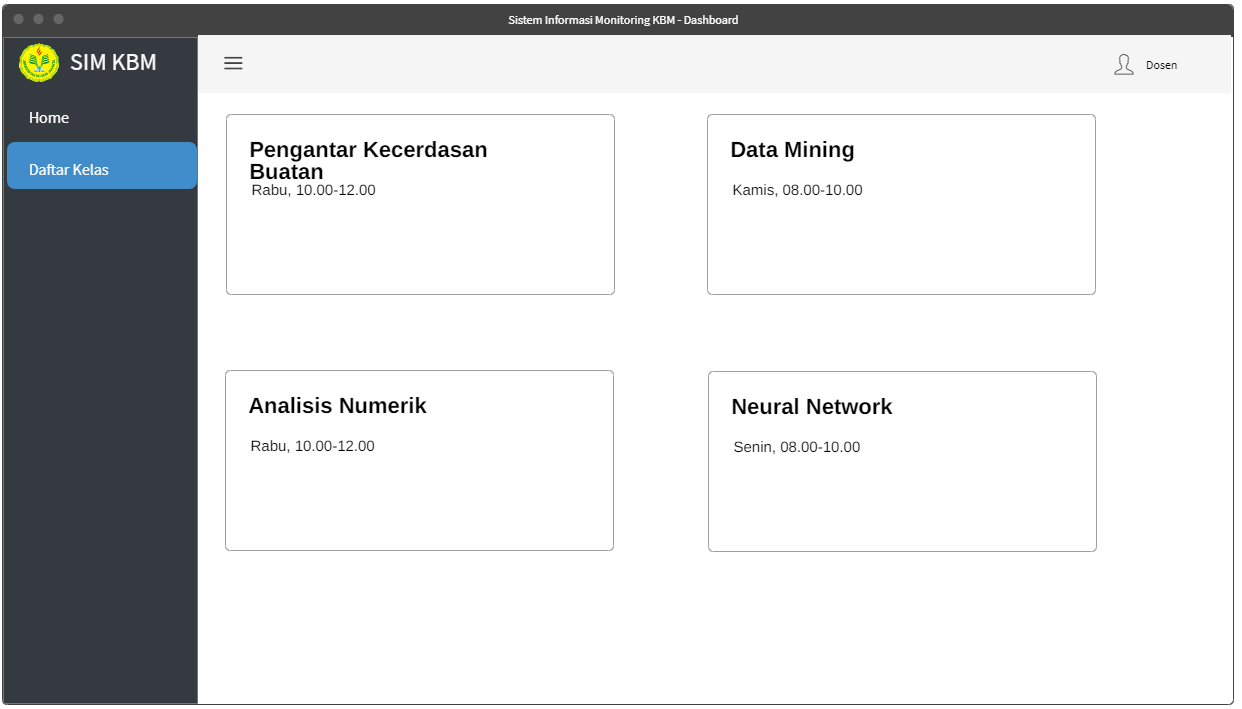
\includegraphics[width=0.8\textwidth]{gambar/mockup/daftar_kelas}
	\caption{Desain Halaman Daftar Kelas}
	\label{fig:daftarkelas}
\end{figure}

\begin{figure}[h!]
	\centering
	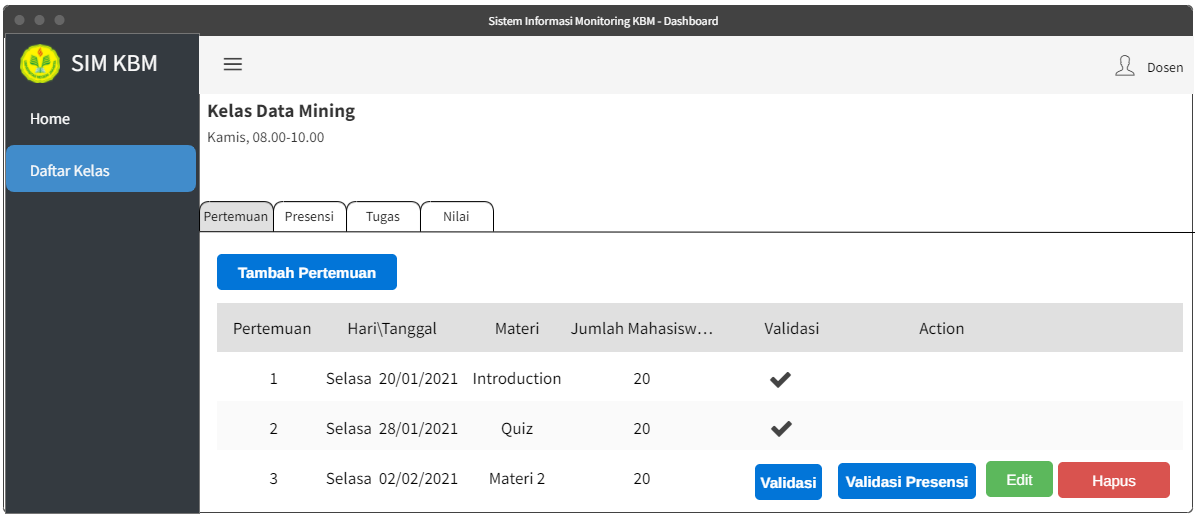
\includegraphics[width=0.8\textwidth]{gambar/mockup/form05_dosen}
	\caption{Desain Halaman Form 05 Pada Dosen}
	\label{fig:form05dosen}
\end{figure}

\begin{figure}[h!]
	\centering
	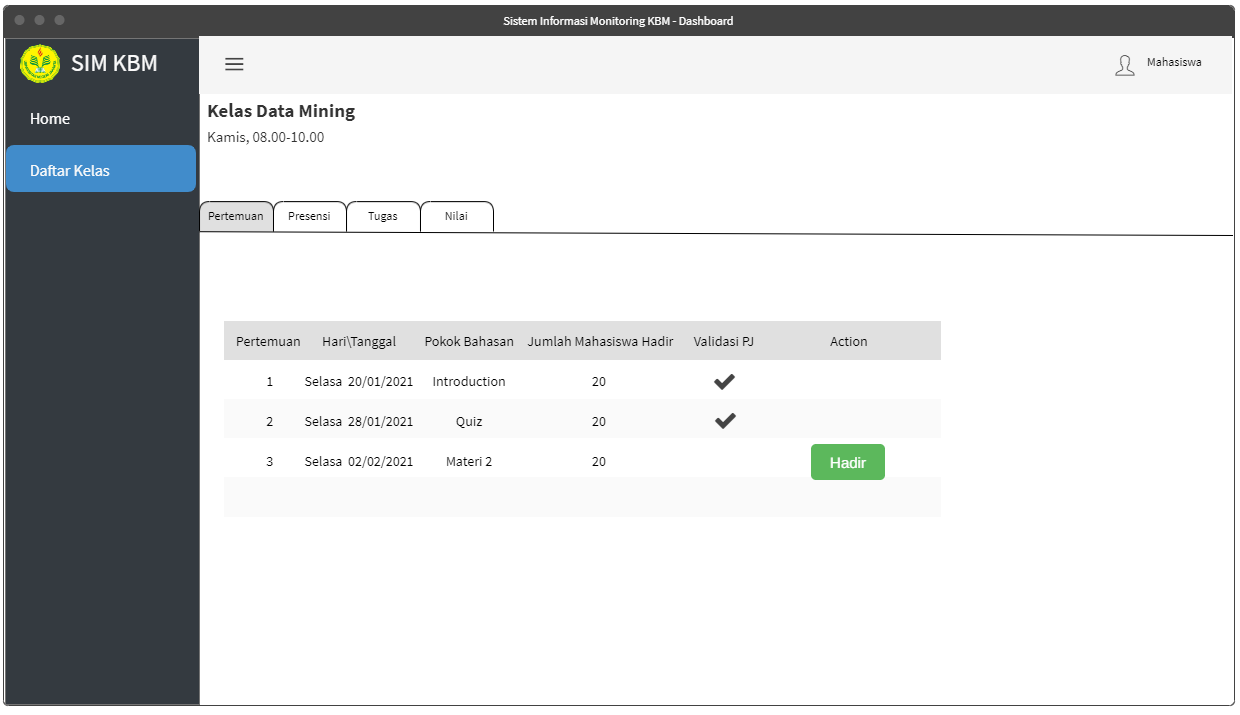
\includegraphics[width=0.8\textwidth]{gambar/mockup/form05_mahasiswa}
	\caption{Desain Halaman Form 05 Pada Mahasiswa }
	\label{fig:form05mhs}
\end{figure}



Pada \textit{tab} presensi yang dapat dilihat pada gambar \ref{fig:presensi}, sistem menampilkan tabel presensi dengan format form 06 dimana setiap presensi yang terekam valid akan ditandai dengan tanda centang, dan presensi kosong akan ditandai dengan tanda silang.

\begin{figure}[h!]
	\centering
	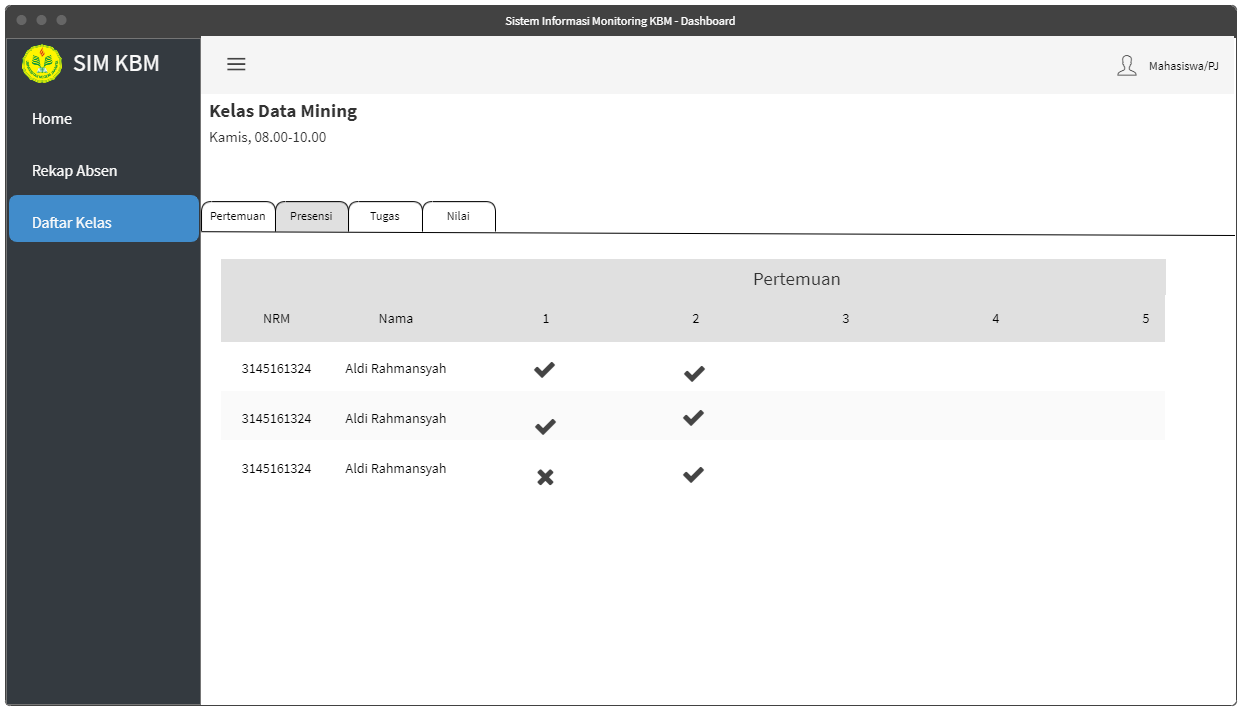
\includegraphics[width=0.8\textwidth]{gambar/mockup/form06_presensi}
	\caption{Desain Halaman Presensi}
	\label{fig:presensi}
\end{figure}

Pada \textit{tab} tugas yang dapat dilihat pada gambar \ref{fig:tugas}, dosen dapat menambah tugas yang diberikan pada mahasiswa atau mengubah tugas yang sudah dibuat sebelumnya. Pada \textit{tab} ini mahasiswa tidak dapat berinteraksi dan hanya dapat melihat tabel tugas tersebut dengan tambahan informasi yaitu nilai pada tugas yang didapatkan tersebut. Tampilan halaman tugas untuk mahasiswa dapat dilihat pada gambar \ref{fig:tugasmhs}

\begin{figure}[h!]
	\centering
	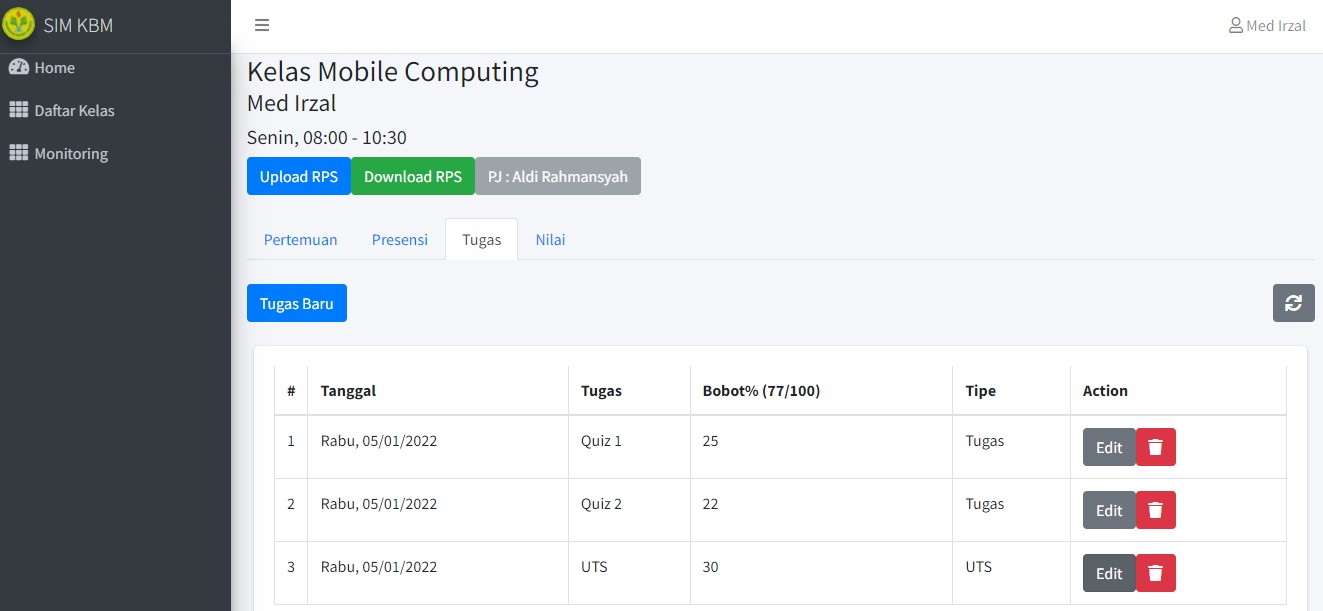
\includegraphics[width=0.8\textwidth]{gambar/mockup/tugas}
	\caption{Desain Halaman Tugas Pada Dosen}
	\label{fig:tugas}
\end{figure}

\begin{figure}[h!]
	\centering
	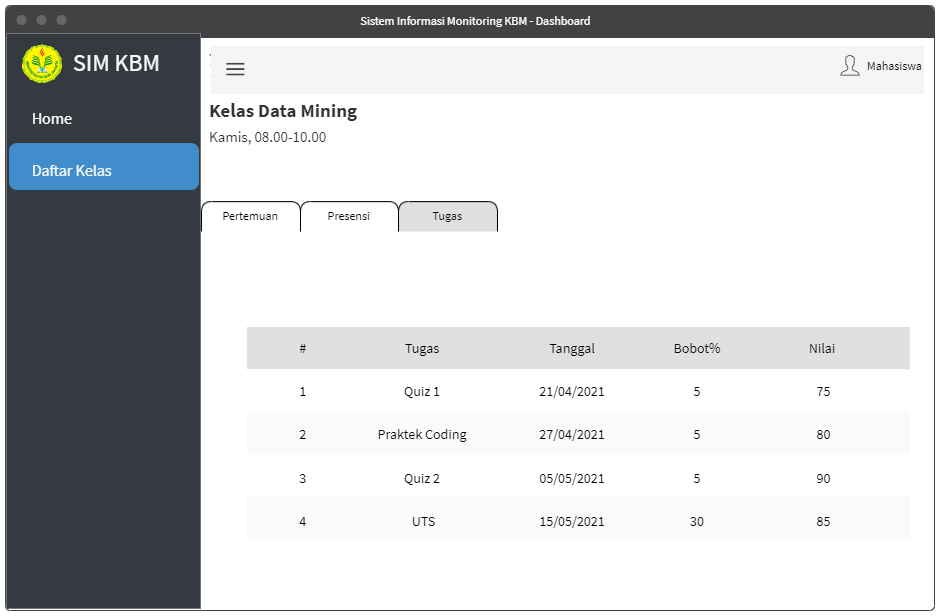
\includegraphics[width=0.8\textwidth]{gambar/mockup/tugas_mahasiswa}
	\caption{Desain Halaman Tugas Pada Mahasiswa}
	\label{fig:tugasmhs}
\end{figure}

Pada \textit{tab} nilai yang dapat dilihat pada gambar \ref{fig:nilai}, dosen dapat melihat tabel nilai setiap mahasiswa dan setiap nilai dari nilai tugas, UTS, dan UAS. Pada \textit{tab} ini, dosen dapat mengunduh dan mengunggah nilai untuk memperbarui nilai pada sistem.

\begin{figure}[h!]
	\centering
	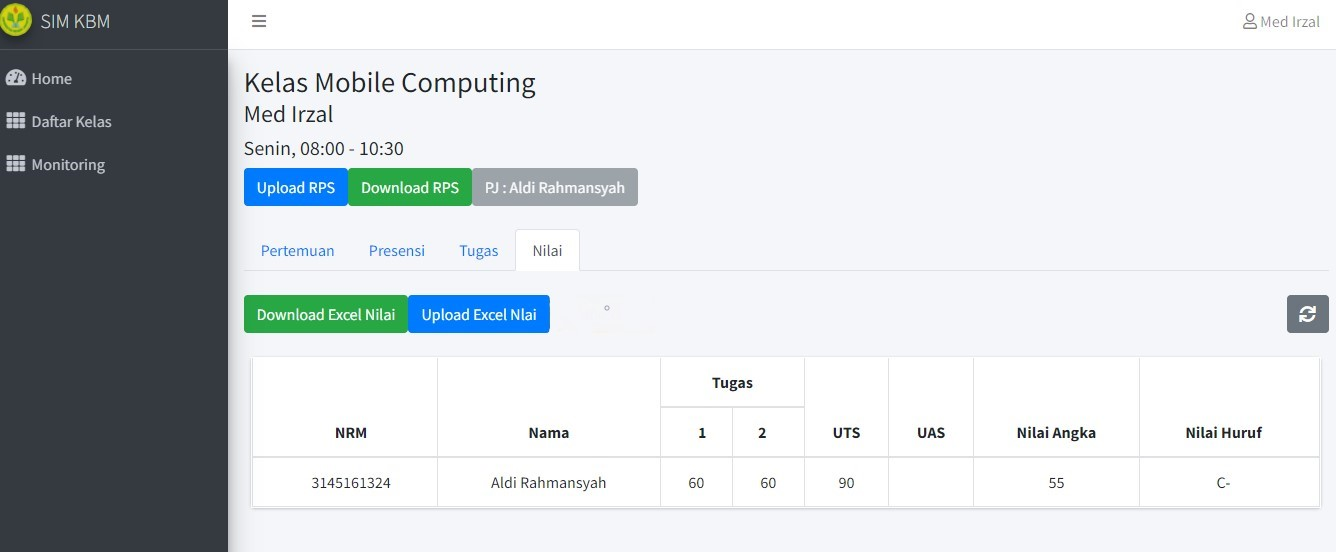
\includegraphics[width=0.8\textwidth]{gambar/mockup/nilai}
	\caption{Desain Halaman Nilai Pada Dosen}
	\label{fig:nilai}
\end{figure}

\end{comment}
%END OF SPS